
\chapter{个人学习Python编码} % Introduction chapter suppressed from the table of contents

第四天早上10:00我终于把所有功能写完并通过自动单元测试!\\
(老师说学编码必须动手,但我平时忙于工作,这次趁十一长假做编码练习题。上次做题已经是春节后,在集中隔离期间做过两题。这次的练习题只有十个功能,本来预计可两天完成。)

\framebox{%
\begin{minipage}[t]{0.97\columnwidth}\raggedright
练习题 (Problem
Set)------分析美国过去温度变化,提供了美国超过20个城市的每天平均温度。(从1961年到2015年)

\begin{itemize}
\tightlist
\item
  先写基本功能:

  \begin{itemize}
  \tightlist
  \item
    画散点图,回归分析,计算标准差与决定系数 (R\textsuperscript{2} Coef.
    of determination)
  \end{itemize}
\end{itemize}

\begin{itemize}
\tightlist
\item
  分析过去的五六十年数据,来判断美国或全球是否在暖化
\end{itemize}

给学生的文件包:

\begin{enumerate}
\tightlist
\item
  ProblemSet5.pdf : 分成 A、 B 、C、 D、
  E部分,详细说明每部分要开发的功能
\item
  PS5.py 程序模板,学员填入代码
\item
  PS5\_test.py 自动单元测试模块,自动测写好的PS5.py
\end{enumerate}\strut
\end{minipage}}


回顾一下,像我这种Python新手,因为不熟悉Python语言的属性与特性,必须按部就班,一步一步来写,欲速则不达。

更重要是体会到个人如何记录数据并分析:

\framebox{%
\begin{minipage}[t]{0.97\columnwidth}\raggedright
\hypertarget{ux8bb0ux5f55ux65f6ux95f4}{%
\subsubsection{记录时间}\label{ux8bb0ux5f55ux65f6ux95f4}}

十多年前我在美国考CMMI培训师,被观察时,
观察老师会在培训后告诉我,每一个模块用了多少时间,与计划对比。
从此以后每次培训我都会习惯记录每个模块所花的时间。

\hypertarget{ux600eux6837ux505a}{%
\subsubsection{怎样做}\label{ux600eux6837ux505a}}

培训时,我都会在桌上放一数字电子钟,记录每一个模块的开始时间与结束时间。上完一天课,晚上在电子表单计划时间旁边写上每个模块的实际时间。
这三天半,我也是用这种方式记录每个模块的时间。

\hypertarget{ux8bb0ux5f55ux7f3aux9677}{%
\subsubsection{记录缺陷}\label{ux8bb0ux5f55ux7f3aux9677}}

因为每个功能都很小,不到20行, 所以没有正式把缺陷与返工工作量记下来。
尤其是一些小的语法错误问题立马就改正了。
但影响较大的重大缺陷,我会记在模块旁边,算是这个模块花的时间。

个人记录实际时间没有想象中这么困难,
只要每天晚上简单按当天本子的数据更新电子表单,避免遗忘。
%will remove after jpg inserted
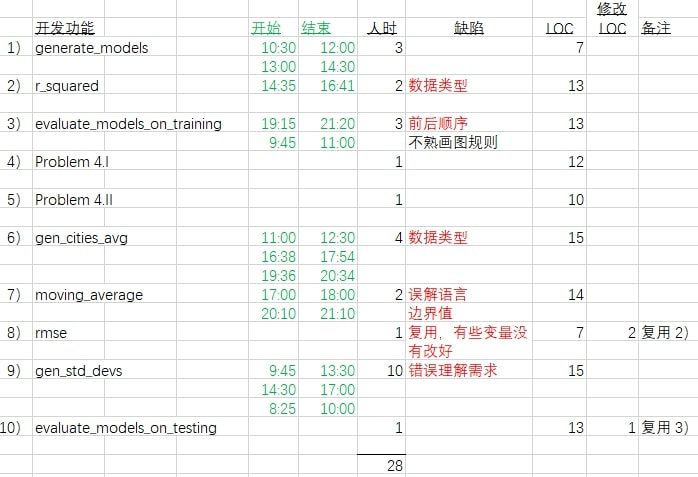
\includegraphics[width=12cm]{PspLogScreenshot_2021-10-06_174917.jpg}
\strut
\end{minipage}}



\framebox{%
\begin{minipage}[t]{0.97\columnwidth}\raggedright
\hypertarget{ux56deux987eux5206ux6790}{%
\subsubsection{回顾分析}\label{ux56deux987eux5206ux6790}}

整个编程结束后,写上每一个模块的实际代码行数。注意:如果模块是复用其他模块代码,便需要注明改动的代码行数。例如:evaluate\_models\_on\_testing13行只修改了1行。

分析:除了标准差模块(gen\_std\_devs)以外,其他功能都能在1-3个小时之内完成。

计算标准差的功能花了 10
小时,问题出在我编码时没有详细看需求。开始以为是求每个城市的温度标准差。
然后再求标准差的平均数。\\
测试不通过后,
也没有再看需求便假定求当年几个城市所有当年每天温度的标准差,还是不对。
到了第四天早上再看看 ProblemSet5.pdf
需求描述才知道我一直误解了这功能需求。

\texttt{gen\_std\_devs~~对应每一输入年份,返回一个数值,依据以下计算:}~\\
\texttt{~1)按输入的所有城市,计算当年每一天的平均温度(所有城市的平均)}~\\
\texttt{~2)计算当年每一天平均温度的标准差}~\\

所以如按我本来的算法,算一个城市是正确,但两个或者多个城市的时候,答案就比正确答案大。

针对这个计算标准差问题,一直以为是语法问题公式计算错误问题。
但我用一些简单的数据检验去,未能发现任何不正常。
来来去去都没有实际的进展,差点想放弃。

\hypertarget{ux7ecfux9a8cux6559ux8bad}{%
\subsubsection{经验教训}\label{ux7ecfux9a8cux6559ux8bad}}

我常常跟客户说,要做好需求评审,才能降低返工工作量。 这次编码实验的经验告诉我,如果前期过程有缺陷遗漏, 后面确实要付出很大的代价。(10小时返工工作量是评审平均2小时(1 - 3小时)的5倍,这案例还只是15行代码的小功能。在实际软件开发项目中,经验丰富的编码员应不像我这么笨,但估计因前面过程遗漏缺陷在系统集成后,测试才发现的返工量应也不止5倍!)

有了数据记录,这类宝贵个人经验便可以转化为改进(不仅仅是一个印象)。例如,可以把这些变成个人风险清单的检查项 
-\/-避免同类问题再发生。

\hypertarget{ux7ed3ux8bba}{%
\subsubsection{结论}\label{ux7ed3ux8bba}}

统计工作量与缺陷数据要从个人开始,并在回顾分析各种缺陷类型的返工量,找根因,制定对应措施,下次可以避免同类缺陷,我们才有动力继续收集数据。\strut
\end{minipage}}


\hypertarget{ux5176ux4ed6ux7f16ux7801ux7ecfux9a8cux6559ux8bad}{%
\subsection{其他编码经验教训}\label{ux5176ux4ed6ux7f16ux7801ux7ecfux9a8cux6559ux8bad}}

\begin{itemize}
\tightlist
\item
  最佳实践: 尽量用最小的行数完成功能

  \begin{itemize}
  \tightlist
  \item
    像Python这类成熟的语言,绝大部分的功能都已经具备
  \item
    尽量避免基础方法编写一个已有的功能(reinvent the
    wheel),除了耗费时间外,还会写多错多
  \end{itemize}
\end{itemize}

\begin{itemize}
\tightlist
\item
  写任何程序前必须先有自动化测试用例

  \begin{itemize}
  \tightlist
  \item
    虽然自己可以先想一些数据自己简单测一下
  \item
    但替代不了另外一个人写的测试用例。跑通才有信心程序正确
    (所以自动单元测试是使用最多的程序)
  \end{itemize}
\end{itemize}

\begin{itemize}
\tightlist
\item
  架构与设计很重要

  \begin{itemize}
  \tightlist
  \item
    校方除了提供测试脚本外,还提供了写程序的模板 (PS5.py)
  \item
    每个功能都明确,输入是什么,什么数据类型,输出是什么
  \item
    学员自己只需要填写实现的代码部分
  \end{itemize}
\end{itemize}

\begin{itemize}
\tightlist
\item
  先把握好新功能的用法与结果

  \begin{itemize}
  \tightlist
  \item
    前面发现不少缺陷,是因为不清楚某功能的用法
  \item
    在写代码之前,自己应开个沙盘,用小程序先试验一下这计算功能有什么参数,会出什么结果
  \end{itemize}
\end{itemize}

\begin{itemize}
\tightlist
\item
  先评审后测试

  \begin{itemize}
  \tightlist
  \item
    在跑程序之前,屏幕展示或打印出刚写好的代码,用铅笔在白纸上按程序的逻辑,从头思考一下每个数据的种类和中间的变化
  \item
    盲目地去跑程序或测试,最终只得出测试失败,但还不清楚错在哪里,如何修改。所以不如在跑程序或测试前,自己先动脑筋模拟一次,仔细想通每个数据的变化
  \end{itemize}
\end{itemize}


